%
% firmware.tex
%
% Copyright The EPS 2.0 Contributors.
%
% EPS 2.0 Documentation
%
% This work is licensed under the Creative Commons Attribution-ShareAlike 4.0
% International License. To view a copy of this license,
% visit http://creativecommons.org/licenses/by-sa/4.0/.
%

%
% \brief Firmware project chapter.
%
% \author Gabriel Mariano Marcelino <gabriel.mm8@gmail.com>
% \author Yan Castro de Azeredo <yan.ufsceel@gmail.com>
%
% \version 0.3.0
%
% \date 2021/03/07
%

\chapter{Firmware} \label{ch:firmware}

\section{Product tree}

The product tree of the firmware part of the EPS 2.0 module is available in \autoref{fig:product-tree-fw}.

\begin{figure}[!ht]
    \begin{center}
        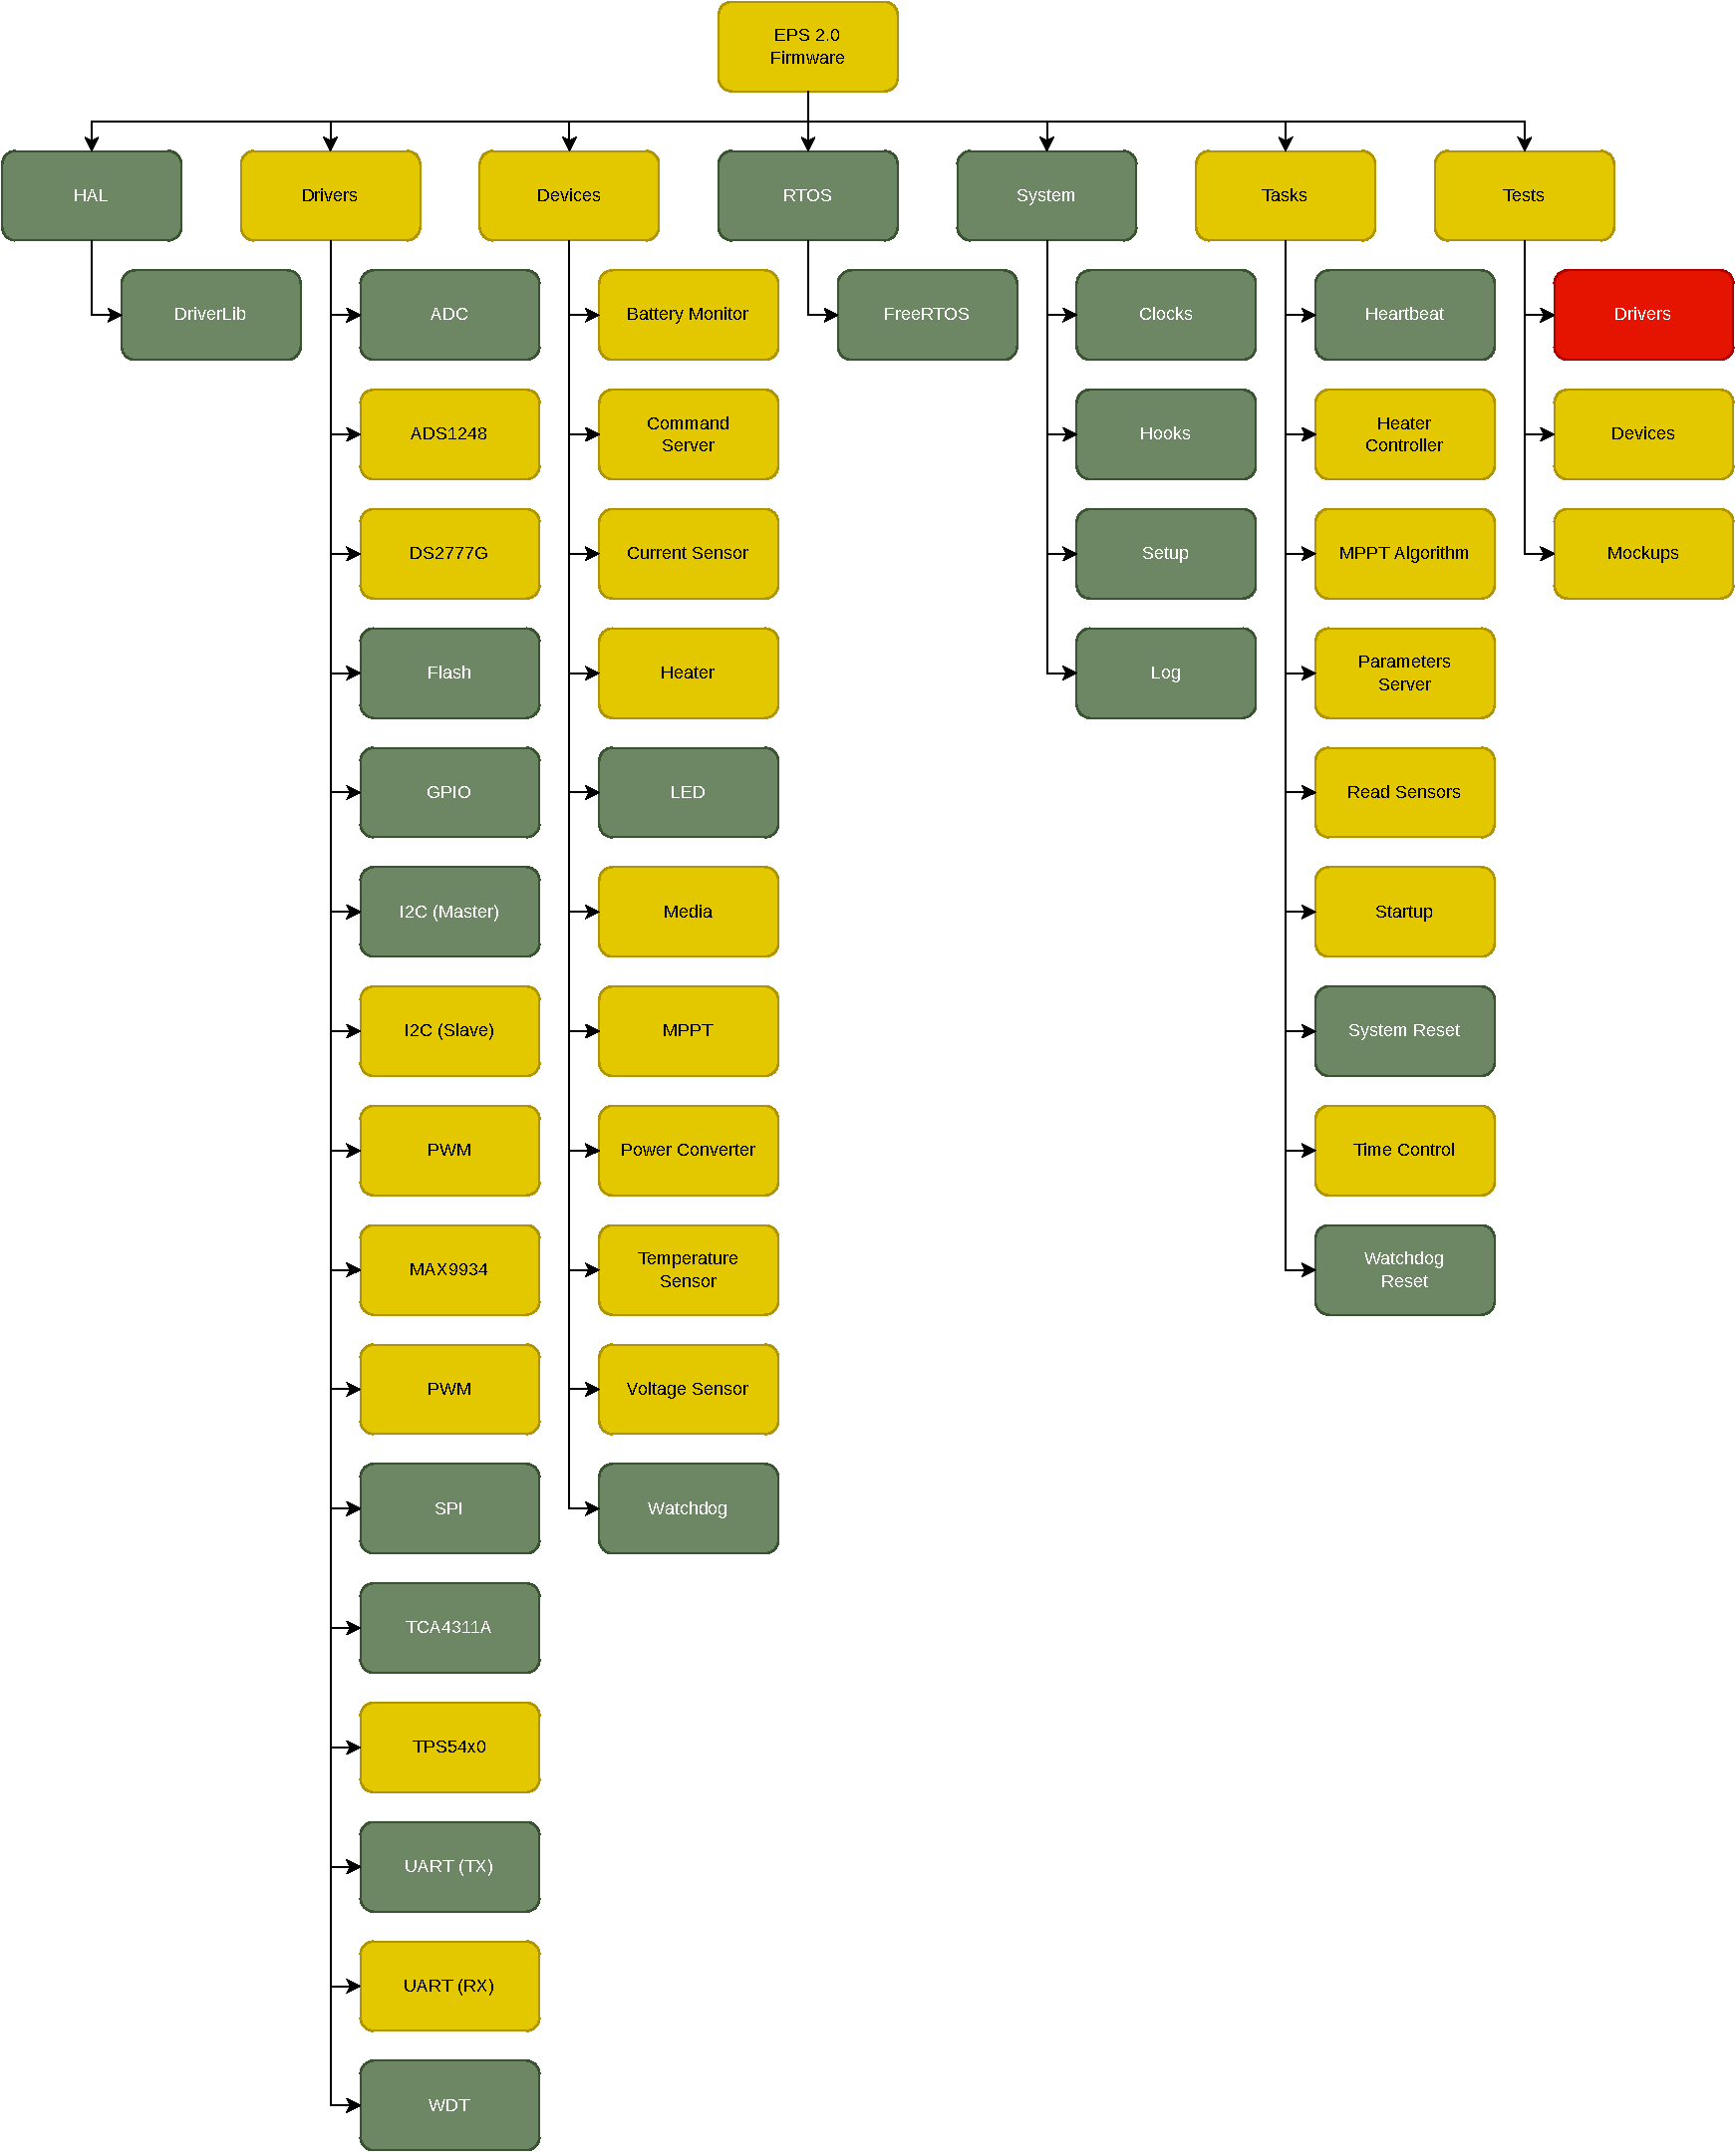
\includegraphics[width=\textwidth]{figures/product-tree-fw.pdf}
        \caption{Product tree of the firmware of the EPS 2.0 module.}
        \label{fig:product-tree-fw}
    \end{center}
\end{figure}

%\section{Dependencies}

\section{Operating System}

The FreeRTOS 10 \cite{freertos} is being used as an operating system. FreeRTOS is a market-leading real-time operating system (RTOS) for microcontrollers and small microprocessors. Distributed freely under the MIT open-source license, FreeRTOS includes a kernel and a growing set of IoT libraries suitable for use across all industry sectors. FreeRTOS is built with an emphasis on reliability and ease of use.

The main configuration parameters of the operating system in this project are available in \autoref{tab:freertos-config}.

\begin{table}[!h]
    \centering
    \begin{tabular}{lrr}
        \toprule[1.5pt]
        \textbf{Parameter}       & \textbf{Value} & \textbf{Unit} \\
        \midrule
        Version                  & v10.2.0        & - \\
        Tick rate (Hz)           & 1000           & Hz \\
        CPU clock (HZ)           & 32             & MHz \\
        Max. priorities          & 5              & - \\
        Heap size                & 40690          & bytes \\
        Max. length of task name & 20             & - \\
        \bottomrule[1.5pt]
    \end{tabular}
    \caption{FreeRTOS main configuration parameters.}
    \label{tab:freertos-config}
\end{table}

More details of the used configuration parameters can be seen in the file \textit{\href{https://github.com/spacelab-ufsc/eps2/blob/master/firmware/config/FreeRTOSConfig.h}{firmware/config/FreeRTOSConfig.h}} from \cite{eps2}.

\section{Hardware Abstraction Layer (HAL)}

As the Hardware Abstraction Layer (HAL\nomenclature{\textbf{HAL}}{\textit{Hardware Abstraction Layer.}}), the DriverLib \cite{driverlib} from Texas Instruments is begin used. It is the official API to access the registers of the MSP430 microcontrollers.

The DriverLib is meant to provide a ``software'' layer to the programmer to facilitate higher level of programming than direct register accesses. By using the high level software APIs provided by DriverLib, users can create powerful and intuitive code that is highly portable between devices within the MSP430 platform and different families in the MSP430/MSP432 platforms.

\section{Tasks}

A list of the firmware tasks can be seen in the \autoref{tab:firmware-tasks}.

\begin{table}[!h]
    \centering
    \begin{tabular}{lccccc}
        \toprule[1.5pt]
        \textbf{name}          & \textbf{priority} & \textbf{initial delay [ms]} & \textbf{period [ms]} & \textbf{stack [bytes]} \\
        \midrule
        startup (boot)         & highest           & 0                           & aperiodic            & 500                    \\
        watchdog reset         & lowest            & 0                           & 100                  & 150                    \\
        heartbeat              & lowest            & 0                           & 500                  & 160                    \\
        system reset           & low               & 0                           & 36000000             & 128                    \\
        heater controller      & medium            & 0                           & 2000                  & 160                    \\
        read sensors           & low               & 0                           & 60000                & 512                    \\
       %csp server             & lowest            & 0                           & 500                  & 1024                   \\
        mppt                   & high              & 0                           & 300                  & 160                    \\
       %beacon package         & tbd               & tbd                         & tbd                  & tbd                    \\
       %obdh package           & highest           & 4500   & called by isr\nomenclature{\textbf{isr}}{\textit{interrupt service routine.}}   & tbd \\
        parameter server       & high              & 0      & called by isr\nomenclature{\textbf{isr}}{\textit{interrupt service routine.}}   & 300 \\
        time control           & high              & 0                           & 1000                 & 128                    \\
        \bottomrule[1.5pt]
    \end{tabular}
    \caption{Firmware tasks.}
    \label{tab:firmware-tasks}
\end{table}

\subsection{Startup (boot)}

This task is responsible for initializing all devices, drivers, libraries, and data structures upon system power-up or reboot.
It is the first task executed and unblocks the remaining tasks after the initialization is completed.

Task configuration parameters are shown in Table \ref{tab:firmware-tasks}.

\subsection{Watchdog reset}

This task is responsible for resetting the internal watchdog timer every \(100 ms\).
The internal watchdog timer has a \(1 s\) timeout.

This task has the lowest possible priority in order to prevent the watchdog from not triggering in case an anomaly happens in other tasks (longer than expected execution times, for example).

Task configuration parameters are shown in Table \ref{tab:firmware-tasks}.

\subsection{Heartbeat}

This task provides visual feedback indicating that the system is running correctly.
This feedback is given through blinking an LED ("SYSTEM\_ON" LED on Figure \ref{fig:status-leds}) at a frequency of \(1 Hz\), emulating a "heartbeat" for the system.

The usefulness of this task comes during the development of the engineering model of the module, providing information to the developers.
The flight model has no LEDs, so this task serves no purpose in that case. 

Task configuration parameters are shown in Table \ref{tab:firmware-tasks}.

\subsection{System reset}

This task is responsible for resetting the microcontroller via software every 10 hours.
This helps to clean up possible corrupted values in variables, retry a failed initialization, clean up RAM, etc.

Task configuration parameters are shown in Table \ref{tab:firmware-tasks}.

\subsection{Heater controller}

This task is responsible for monitoring and controlling the batteries' heaters.

The heaters and batteries' temperatures are monitored through a set of RTDs, read through an external ADC (\textit{ADS1248}), and activated through MOSFET drivers controlled by the MCUs GPIOs to prevent the batteries from operating below a critical temperature value.

This task has two modes of operation, automatic mode, and manual mode.

In automatic mode, the batteries' temperature readings occur every 2 seconds. The heaters' status is updated accordingly, based on the new reading and a predefined temperature limit, through the algorithm defined in the heater device.
This algorithm switches the heaters on or off based on the set temperature limits.

In manual mode, the heater is controlled manually through telecommands, independent of the temperature readings. In this mode, the heaters are controlled with a PWM signal with a duty cycle defined via telecommand.

Task configuration parameters are shown in Table \ref{tab:firmware-tasks}.

\subsection{Read sensors}

This task is responsible for reading all sensors available to the EPS 2.0 module and recording their values.
The readings occur every \(60 s\), and the results are written in the eps buffer data structure.

Task configuration parameters are shown in Table \ref{tab:firmware-tasks}.

\subsection{MPPT}

This task is responsible for running the MPPT algorithm for the solar panels to operate them at their maximum power point.
The algorithm itself is defined in the MPPT device.

The solar panels' current and voltage sensors are read every \(300 ms\), and the results are passed as inputs to the MPPT algorithm, which then controls the MPPT Boost circuit through a set o PWM outputs.

The MPPT task can also operate in manual mode, where the PWM outputs are set manually via telecommands.

Task configuration parameters are shown in Table \ref{tab:firmware-tasks}.

\subsection{Parameter Server}

This task is responsible for processing and responding to commands from the OBDH and TTC modules.

The commands are for reading and writing to the EPS buffer data structure, seen in \autoref{tab:eps2-variables}

Task configuration parameters are shown in Table \ref{tab:firmware-tasks}.

\subsection{Time Control}

This task is responsible for the time management of the system.
At every second, it increments the system time (epoch).
Also, it saves the current system time in the non-volatile memory at every minute.

Task configuration parameters are shown in Table \ref{tab:firmware-tasks}.

% \subsection{Beacon package}

% Task configuration parameters are shown in Table \ref{tab:firmware-tasks}.

% \subsection{OBDH package}

% Task configuration parameters are shown in Table \ref{tab:firmware-tasks}.

\section{Variables and Parameters}

A list of all the variables of EPS with their identification number (ID) and variable type that can be read from the sensors and peripherals is seen in the \autoref{tab:eps2-variables}.

\begin{longtable}[c]{cL{0.72\textwidth}lc}
    \toprule[1.5pt]
    \textbf{ID} & \textbf{Name/Description} & \textbf{Type} & \textbf{Access} \\
    \midrule
    0   & Time counter in milliseconds                                       & uint32 & R \\
    1   & Temperature of the $\mu$C in K                                    & uint16 & R \\
    2   & EPS circuitry current in mA                                       & uint16 & R \\
    \multirow{18}{*}{3} & Last reset cause: & \multirow{18}{*}{uint8} & \multirow{18}{*}{R} \\
        & - 0x00 = No interrupt pending                                     &        &  \\
        & - 0x02 = Brownout (BOR)                                           &        &  \\
        & - 0x04 = RST/NMI (BOR)                                            &        &  \\
        & - 0x06 = PMMSWBOR (BOR)                                           &        &  \\
        & - 0x08 = Wakeup from LPMx.5 (BOR)                                 &        &  \\
        & - 0x0A = Security violation (BOR)                                 &        &  \\
        & - 0x0C = SVSL (POR)                                               &        &  \\
        & - 0x0E = SVSH (POR)                                               &        &  \\
        & - 0x10 = SVML\_OVP (POR)                                          &        &  \\
        & - 0x12 = SVMH\_OVP (POR)                                          &        &  \\
        & - 0x14 = PMMSWPOR (POR)                                           &        &  \\
        & - 0x16 = WDT time out (PUC)                                       &        &  \\
        & - 0x18 = WDT password violation (PUC)                             &        &  \\
        & - 0x1A = Flash password violation (PUC)                           &        &  \\
        & - 0x1C = Reserved                                                 &        &  \\
        & - 0x1E = PERF peripheral/configuration area fetch (PUC)           &        &  \\
        & - 0x20 = PMM password violation (PUC)                             &        &  \\
        & - 0x22 to 0x3E = Reserved                                         &        &  \\
    4   & Reset counter                                                     & uint16 & R \\
    5   & -Y and +X sides solar panel voltage in mV                         & uint16 & R \\
    6   & -X and +Z sides solar panel voltage in mV                         & uint16 & R \\
    7   & -Z and +Y sides solar panel voltage in mV                         & uint16 & R \\
    8   & -Y side solar panel current in mA                                 & uint16 & R \\
    9   & +Y side solar panel current in mA                                 & uint16 & R \\
    10  & -X side solar panel current in mA                                 & uint16 & R \\
    11  & +X side solar panel current in mA                                 & uint16 & R \\
    12  & -Z side solar panel current in mA                                 & uint16 & R \\
    13  & +Z side solar panel current in mA                                 & uint16 & R \\
    14  & MPPT 1 duty cycle in \% (writable just in manual mode)            & uint8  & R/W \\
    15  & MPPT 2 duty cycle in \% (writable just in manual mode)            & uint8  & R/W \\
    16  & MPPT 3 duty cycle in \% (writable just in manual mode)            & uint8  & R/W \\
    17  & Total solar panels output voltage after MPPT in mV                & uint16 & R \\
    18  & Main power bus voltage in mV                                      & uint16 & R \\
    19  & RTD0 temperature in K                                             & uint16 & R \\
    20  & RTD1 temperature in K                                             & uint16 & R \\
    21  & RTD2 temperature in K                                             & uint16 & R \\
    22  & RTD3 temperature in K                                             & uint16 & R \\
    23  & RTD4 temperature in K                                             & uint16 & R \\
    24  & RTD5 temperature in K                                             & uint16 & R \\
    25  & RTD6 temperature in K                                             & uint16 & R \\
    26  & Batteries voltage in mV                                           & uint16 & R \\
    27  & Batteries current in mA                                           & uint16 & R \\
    28  & Batteries average current in mA                                   & uint16 & R \\
    29  & Batteries accumulated current in mA                               & uint16 & R \\
    30  & Batteries charge in mAh                                           & uint16 & R \\
    31  & Battery monitor IC temperature in K                               & uint16 & R \\
    32  & Battery monitor status register                                   & uint8  & R \\
    33  & Battery monitor protection register                               & uint8  & R \\
    34  & Battery monitor cycle counter                                     & uint8  & R \\
    35  & Battery monitor Remaining Active-Absolute Capacity (RAAC) in mAh  & uint16 & R \\
    36  & Battery monitor Remaining Standby-Absolute Capacity (RSAC) in mAh & uint16 & R \\
    37  & Battery monitor Remaining Active-Relative Capacity (RARC) in \%   & uint8  & R \\
    38  & Battery monitor Remaining Standby-Relative Capacity (RSRC) in \%  & uint8  & R \\
    39  & Battery heater 1 duty cycle in \% (writable just in manual mode)  & uint8  & R/W \\
    40  & Battery heater 2 duty cycle in \% (writable just in manual mode)  & uint8  & R/W \\
    41  & Hardware version                                                  & uint8  & R \\
    42  & Firmware version (ex.: ``v1.2.3''' = 0x00010203)                  & uint32 & R \\
    43  & MPPT 1 mode (0x00 = automatic, 0x01 = manual)                     & uint8  & R/W \\
    44  & MPPT 2 mode (0x00 = automatic, 0x01 = manual)                     & uint8  & R/W \\
    45  & MPPT 3 mode (0x00 = automatic, 0x01 = manual)                     & uint8  & R/W \\
    46  & Battery heater 1 mode (0x00 = automatic, 0x01 = manual)           & uint8  & R/W \\
    47  & Battery heater 2 mode (0x00 = automatic, 0x01 = manual)           & uint8  & R/W \\
    48  & Device ID (0xEEE2)                                                & uint16 & R \\
    \bottomrule[1.5pt]
    \caption{Variables and parameters of the EPS 2.0.}
    \label{tab:eps2-variables}
\end{longtable}

